\documentclass{article} %======================================================

% package includes
\usepackage[polish]{babel}  %polish typhographical rules
\usepackage[utf8]{inputenc} %input in in UTF-8
\usepackage{polski}         %more polish in this document
\usepackage[T1]{fontenc}    %font encoding
\usepackage{url}            %URL formatting
\usepackage{xcolor}         %some color definitions
\usepackage{indentfirst}    %indent at the beginning of each paragraph
\usepackage{graphicx}       %image insertion package
\usepackage{listings}       %for shell commands listing

%use some polish typhographical rules borrowed from french
\frenchspacing

%redefine page geometry (margins)
\addtolength{\textwidth}{3cm}
\addtolength{\hoffset}{-1.5cm}
\addtolength{\textheight}{3cm}
\addtolength{\voffset}{-1.5cm}

%define style for bash command listing
\lstdefinestyle{bash}{
    language=bash,                         %listings are in bash
    basicstyle=\small\ttfamily,            %basic text style (\sffamily)
    stringstyle=\ttfamily,                 %typewriter type for strings
    numbers=none,                          %no line numbers
%    numberstyle=\tiny,
%    numbersep=3pt,
    showstringspaces=false,                %no special characters instead of spaces
    keywordstyle=,%\color{black}\bfseries, %normally keywords would be typed in bold, but since listings package determines keywords wrongly, their style is the same as basic style
    frame=tb,                              %top and bottom border
    columns=fullflexible,                  %fixed columns would make listings not fit into page width
    backgroundcolor=\color{gray!20},       %some nice background color
    linewidth=1.0\linewidth,
    xleftmargin=0.0\linewidth
}

\begin{document} %=============================================================

\title{Apache Cassandra 2.0\\\vspace{2ex}Przewodnik instalacji i konfiguracji w systemie Debian Wheezy\\\vspace{3ex}}
\author{Jan Baranowski, Michał Kaik\\Politechnika Poznańska}

\maketitle

\section{Wstęp}\label{sec:intro}

Niniejszy dokument ma za zadanie przedstawić proces instalacji i~konfiguracji serwera baz danych NoSQL \emph{Apache Cassandra} w~środowisku rozproszonym.
Na potrzeby demonstracji zakłada się że środowisko to będzie składać się z kilku węzłów połączonych siecią lokalną.

\emph{Apache Cassandra} jest serwerem baz danych NoSQL, początkowo rozwijanym przez \emph{Facebooka} na potrzeby umożliwienia efektywnego wyszukiwania wiadomości w~skrzynce odbiorczej.
Obecnie (od marca 2009 roku) \emph{Cassandra} jest rozwijana przez \emph{Apache Foundation} (jako jeden z~projektów top-level) i~stanowi podstawę dla zestawu narzędzi DataStax. 

\emph{Cassandra} powstała jako narzędzie mające w~założeniu cechować się:
\begin{itemize}
\item wysoką dostępnością (\emph{Cassandra} jest określana jako zawsze zapisywalna baza danych)
\item niskim opóźnieniem wykonywanych operacji (\textit{ang.}~latency)
\item odpornością na awarie (możliwością replikacji danych, brakiem komponentów, których awaria może zdestabilizować system (\textit{ang.}~single points of failure))
\item możliwością regulacji kompromisu pomiędzy szybkością działania a~odpornością na awarie i~spójnością replik
\item relatywnie prostym modelem danych
\end{itemize}

Zarówno opisanie kolumnowego modelu danych wykorzystywanego w~\emph{Cassandrze}, jak i~mechanizmów, dzięki którym spełnia ona założenia projektowe nie jest celem tego dokumentu.
Autorzy mogą jedynie podać propozycje publikacji, które opisują wspomniane zagadnienia.
Zarówno dla modelu danych, jak i~budowy wewnętrznej \emph{Cassandry} będzie to przede wszystkim dokumentacja udostępniana przez firmę \emph{DataStax} \cite{datastax}.
Kolumnowy model danych, przedstawiony z~perspektywy osób pracujących z~bazami relacyjnymi został doskonale (choć może zbyt obszernie) opisany w~\emph{Cassandra --- The Definitive Guide} \cite{definitiveguide}.
Z~kolei architektura \emph{Cassandry} w~dużym skrócie (choć zapewne w~sposób wystarczający by służyć jako wstęp do tego dokumentu) została przedstawiona w~prezentacji \cite{prezentacja_srds}.

Procedurę przygotowania klastra przedstawiono na przykładzie systemu operacyjnego Debian GNU/Linux 6, ponieważ uchodzi on za jedno z~lepszych rozwiązań dla serwerów.

\section{Wybór dystrybucji}\label{sec:distro}

Na samym początku nowi użytkownicy \emph{Cassandry} stają przed wyborem dystrybucji tego oprogramowania.
Możliwości są dwie: instalacja standardowej wersji dostarczonej przez \emph{Apache Foundation} oraz instalacja platformy \emph{DataStax}~---~zestawu narzędzi obudowujących \emph{Cassandrę} i~dostarczających m.in. funkcje pozwalające na uproszczenie zarządzania klastrem, wizualne monitorowanie, analizę obciążeń węzłów, itp. (por. rysunek \ref{fig:datastax_arch}).

\begin{figure}[h]
\centering
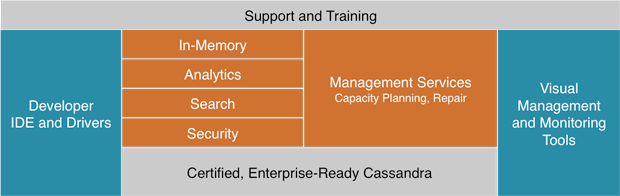
\includegraphics[width=\linewidth]{gfx/datastax}
\caption{architektura \emph{DataStax} w~odniesieniu do \emph{Cassandry}, źródło:~\cite{whydatastax}}
\label{fig:datastax_arch}
\end{figure}

Wybór jest ważny o~tyle, że pomimo wspólnego fundamentu, jakim jest \emph{Cassandra}, procesy instalacji obu dystrybucji nie mają ze sobą nic wspólnego, tj. (według wiedzy autorów) nie da się doinstalować do dystrybucji \emph{Apache} platformy \emph{DataStax}.

W~tym miejscu należy wspomnieć o~twórcach platformy~---~firmie o~zaskakującej nazwie \emph{DataStax}, zajmującej się dostosowaniem \emph{Cassandry} do potrzeb przedsiębiorstw poprzez m.in. rozwój i~testowanie bazy danych, dostarczanie narzędzi ułatwiających administrację systemem, organizację szkoleń, certyfikację personelu technicznego, itd.
Bodaj najbardziej znaczącym wkładem \emph{DataStax} w~rozwój projektu jest opracowanie szeregu driverów/konektorów dla różnych języków programowania, dzięki którym programiści mogą korzystać z~\emph{Cassandry} w~sposób analogiczny do rozwiązań relacyjnych (np. tak jak w~przypadku \emph{MySQL Connectors}, por. \cite{mysql_connectors}) i~rozbudowa dokumentacji technicznej platformy, włączając w~to dokumentację plików konfiguracyjnych, architektury \emph{Cassandry} i języka \emph{CQL} (odpowiednika \emph{SQL} dla kolumnowych baz danych).

Na potrzeby niniejszego dokumentu założono, że właściwym wyborem będzie dystrybucja \emph{Apache Cassandra}, ze względu na to, że dokument ma pełnić rolę wprowadzenia do technologii, nie zaś pozwalać na błyskawiczne wdrożenie systemu (\textit{ang.}~rapid deployment).
Poza tym, przewodniki instalacji i~konfiguracji \emph{DataStaxa} dostępne są np. na stronie \cite{datastax_guides}.

\section{Instalacja}\label{sec:install}

\emph{Cassandra} zostanie zainstalowana przy użyciu narzędzia \emph{APT} z~repozytorium \emph{Apache Software Foundation}.
Wymagane będzie dodanie odpowiedniego repozytorium do listy źródeł \emph{APTa}.
Dodatkowo ze względu na to, że \emph{Cassandra} napisana jest w~Javie, pokazany zostanie proces instalacji \emph{Oracle JRE} w~systemie \emph{Debian} (ta maszyna wirtualna jest zalecana przez twórców \emph{Cassandry}).

\subsection{Wybór maszyny wirtualnej Java}\label{subsec:install_vm}

\emph{Apache Software Foundation} dostarcza pakiety zawierające \emph{Cassandrę} w~formacie \texttt{*.deb}, a~także repozytorium dla \emph{APTa}.
Jedną z~zależności pakietu \texttt{cassandra} jest pakiet \texttt{openjdk-7-jre}.
Jest to w~pewnym sensie sprzeczne z~zaleceniami twórców bazy danych, ponieważ ci rekomendują maszynę wirtualną \emph{Oracle} jako środowisko uruchomieniowe (nawet w~testowanej wersji bazy 2.0 odpowiedni komunikat wyświetlany jest w~logu).
Nie zmienia to faktu, że testy (funkcjonalne, lecz nie wydajnościowe) przeprowadzone na potrzeby tego artykułu udowodniły, że \emph{Cassandra} działa bez zarzutu także w~środowisku \emph{OpenJDK}. 

Należy zatem wybrać pomiędzy stosowaniem się do zaleceń a~prostotą instalacji.

\subsection{Instalacja i konfiguracja Oracje Java}\label{subsec:install_oracle}

Pakiet z~\emph{OpenJDK} jest instalowany jako pakiet zależny podczas instalacji Cassandry.
Jeżeli jednak administrator zdecyduje się użyć \emph{Oracle JVM}, poniżej przedstawiona jest skrótowa procedura instalacji tego oprogramowania w~systemie \emph{Debian}.
Stanowi ona kompilację najprostszych rozwiązań i~tym różni się od większości przewodników dostępnych w~internecie, że poza konsolą systemu nie wymaga żadnych dodatkowych narzędzi (np. mechanizmu transferu plików z~maszyny-terminala do maszyny-serwera).

Pierwszym krokiem jest pobranie pakietu oprogramowania (JRE, nie JDK) ze strony \emph{Oracle}.
Standardowo by pobrać plik należy zaakceptować umowę licencyjną, jednak przy odpowiedniej konfiguracji możliwe jest ominięcie tego kroku \cite{downloading_oracle_java}:

\begin{lstlisting}[style=bash, caption={pobieranie \emph{Oracle JRE}}]
$ wget --no-cookies \
> --no-check-certificate \
> --header "Cookie: oraclelicense=accept-securebackup-cookie" \
> "http://download.oracle.com/otn-pub/java/jdk/7u60-b19/jre-7u60-linux-i586.tar.gz" \
> -O /tmp/jre-7u60-linux-i586.tar.gz
\end{lstlisting}

Popularnym sposobem instalacji pobranego oprogramowania jest wypakowanie archiwum (zazwyczaj do katalogu \texttt{/opt}) i~ręczna konfiguracja ścieżki systemowej (por. \cite{downloading_oracle_java}).
\emph{Debian} dostarcza jednak narzędzie pozwalające przekonwertować archiwum do pakietu \emph{DEB} \cite{installing_oracle_java_on_debian}.

Należy je zainstalować, a~potem użyć:

\begin{lstlisting}[style=bash, caption={budowa pakietu DEB z~\emph{Oracle JRE}}]
$ apt-get install java-package

$ fakeroot make-jpkg /tmp/jre-7u60-linux-i586.tar.gz
\end{lstlisting}

Powstały w~ten sposób pakiet \emph{DEB} należy zainstalować.
Po instalacji należy ustawić \emph{Oracle JVM} jako domyślną maszynę wirtualną w~systemie.

\begin{lstlisting}[style=bash, caption={instalacja i konfiguracja \emph{Oracle JRE}}]
$ dpkg -i /tmp/oracle-j2re1.7_1.7.0+update60_i386.deb

$ update-alternatives --config java
There are 2 choices for the alternative java (providing /usr/bin/java).

  Selection    Path                                           Priority   Status
------------------------------------------------------------
  0            /usr/lib/jvm/java-7-openjdk-i386/jre/bin/java   1051      auto mode
* 1            /usr/lib/jvm/j2re1.7-oracle/bin/java            316       manual mode
  2            /usr/lib/jvm/java-7-openjdk-i386/jre/bin/java   1051      manual mode

Press enter to keep the current choice[*], or type selection number:

$ java -version
java version "1.7.0_60"
Java(TM) SE Runtime Environment (build 1.7.0_60-b19)
Java HotSpot(TM) Client VM (build 24.60-b09, mixed mode)
\end{lstlisting}

Według wiedzy autorów Cassandra nie wymaga ustawiania zmiennej \lstinline[style=bash]!JAVA_HOME! dla żadnego z użytkowników (ani roota, ani użytkownika \textit{cassandra}, właściciela demona). Jeżeli jednak zajdzie taka potrzeba, zainstalowane maszyny wirtualne można znaleźć w katalogu /usr/lib/jvm.

\begin{lstlisting}[style=bash, caption={ustawianie JAVA\textunderscore HOME}]
$ echo "export JAVA_HOME=/usr/lib/jvm/j2re1.7-oracle/" >> /home/<user>/.bashrc
\end{lstlisting}

\subsection{Konfiguracja repozytorium}\label{subsec:install_repo}

By móc zainstalować \emph{Cassandrę}, należy dodać odpowiednie repozytorium \emph{Apache Software Foundation} do źródeł programu \emph{APT}.
Zgodnie z~konwencją każda większa wersja \emph{Cassandry} znajduje się w~osobnym repozytorium.
Na potrzeby tego dokumentu w systemie testowym zostanie zainstalowana \emph{Cassandra 2.0.8}.

Do pliku \texttt{/etc/apt/sources.list} należy dopisać:

\begin{lstlisting}[style=bash, caption={nowe źródła pakietów dla \emph{APTa}}]
deb http://www.apache.org/dist/cassandra/debian 20x main
deb-src http://www.apache.org/dist/cassandra/debian 20x main
\end{lstlisting}

Próba pobrania spisu zawartości repozytorium zakończy się niepowodzeniem, ponieważ \emph{APT} nie zna kluczy publicznych dla repozytorium \emph{Apache Software Foundation}.
Te należy dodać w~następujący sposób:

\begin{lstlisting}[style=bash, caption={pobieranie kluczy publicznych repozytorium \emph{ASF}}]
$ gpg --keyserver pgp.mit.edu --recv-keys F758CE318D77295D
$ gpg --export --armor F758CE318D77295D | sudo apt-key add -

$ gpg --keyserver pgp.mit.edu --recv-keys 2B5C1B00
$ gpg --export --armor 2B5C1B00 | sudo apt-key add -
\end{lstlisting}

Po zakończeniu wszystkich operacji należy pobrać spis zawartości repozytoriów:
\begin{lstlisting}[style=bash, caption={odświeżanie list pakietów}]
$ apt-get update
\end{lstlisting}

\subsection{Instalacja Cassandry}\label{subsec:install_install}

Ostatnim krokiem procesu instalacji jest zainstalowanie \emph{Cassandry} z~użyciem \emph{APTa}:
\begin{lstlisting}[style=bash, caption={instalacja \emph{Cassandry}}]
$ apt-get install cassandra
\end{lstlisting}

W~efekcie \emph{Cassandra} powinna zostać zainstalowana i~uruchomiona.

\section{Konfiguracja węzła}\label{sec:config}

Ta część dokumentu opisuje czynności związane z~konfiguracją węzła \emph{Cassandry} tak, by był on zdolny dołączyć do klastra.
\emph{Cassandra} jest systemem P2P, więc o~utworzeniu klastra węzły decydują wspólnie w~oparciu o~taką samą nazwę klastra zdefiniowaną w~pliku konfiguracyjnym i~włączony kanał komunikacji poprzez plotkowanie.
Kanał ten jest domyślnie wyłączony, zatem każdy węzeł \emph{Cassandry} w~sieci będzie z~początku tworzył osobny klaster.

\subsection{Stan systemu po instalacji}\label{subsec:config_postinst}

Zaraz po instalacji w~systemie pojawia się nowa usługa: \texttt{cassandra}.
Jest ona domyślnie uruchomiona.
Jej konfiguracja zapobiega możliwości dołączenia węzła do jakiegokolwiek klastra ze względu na zablokowanie mechanizmu plotkowania (dokładnie: agent implementujący algorytm plotkujący nasłuchuje wyłącznie na adresie IP 127.0.0.1).

Pliki konfiguracyjne można znaleźć w~katalogu \texttt{/etc/cassandra}.
Są wśród nich:

\begin{itemize}
\item \texttt{/etc/cassandra/cassandra-env.sh}~---~skrypt definiujący zmienne środowiskowe w formie argumentów dla maszyny wirtualnej Java (np. wielkość stosu, ale także m.in. włączenie/wyłączenie mechanizmu \emph{JMX}).
\item \texttt{/etc/cassandra/cassandra-rackdc.properties}~---~informacja o tym, w~którym fizycznie racku i~centrum danych znajduje się obecny węzeł.
\item \texttt{/etc/cassandra/cassandra-topology.properties}~---~przybliżone informacje o tym, w~których rackach i~centrach danych znajdują się inne węzły klastra. Plik ten jest wykorzystywany przez jedną z~kilku wersji algorytmu rozmieszczania replik (\emph{snitcha}).
\item \texttt{/etc/cassandra/cassandra-topology.yaml}~---~plik analogiczny do poprzedniego, wykorzystywany jednak przez inną wersję algorytmu.
\item \texttt{/etc/cassandra/cassandra.yaml}~---~główny plik konfiguracyjny \emph{Cassandry}.
\end{itemize}

Pliki danych (w~tym: commit logi) znaleźć można w~katalogu \texttt{/var/lib/cassandra}.
Czyszcząc zawartość trzech znajdujących się w~nim podkatalogów można zresetować stan klastra.
W~celu wykonania tej czynności autorzy nie zalecają jednak ich całkowitego usuwania (podczas testowania mogą one zostać utworzone na nowo z~prawem zapisu tylko dla roota, co uniemożliwi normalny start usługi).

Plik logu znaleźć można w~\texttt{/var/log/cassandra/system.log}.

\subsection{Jak debugować konfigurację?}\label{subsec:config_debug}

Przed rozpoczęciem wprowadzania zmian do plików konfiguracyjnych zaleca się wyłączenie automatycznego uruchamiania usługi.
Błędnie skonfigurowany węzeł może dołączyć do nieodpowiedniego klastra, a~jego usunięcie w~takim przypadku nie jest zadaniem trywialnym.
Efekt można osiągnąć wykonując polecenie:

\begin{lstlisting}[style=bash, caption={wyłączenie uruchamiania \emph{Cassandry} na jej domyślnych runlevelach}]
$ insserv -r cassandra
\end{lstlisting}

Najprostszym sposobem sprawdzenia poprawności konfiguracji jest uruchomienie węzła w~trybie jawnym (w~przeciwieństwie do deamona).
Służy do tego podane poniżej polecenie, które wypisze log działania węzła na standardowe wyjście.

\begin{lstlisting}[style=bash, caption={testowe uruchamianie \emph{Cassandry}}]
$ cassandra -f  # -f for foreground
\end{lstlisting}

Dodatkowo można zarchiwizować taki log poleceniem \texttt{tee plik.log}, które skopiuje standardowe wejście na standardowe wyjście i do podanego pliku:

\begin{lstlisting}[style=bash, caption={testowe uruchamianie \emph{Cassandry} z archiwizacją logu}]
$ cassandra -f | tee /tmp/cassandra_testrun.log
\end{lstlisting}

\bigskip

\noindent\textbf{UWAGA!} Jeżeli \emph{Cassandra} zostanie uruchomiona w~trybie jawnym podczas gdy równolegle usługa działa w~tle, zamiast informacji o~błędzie w~logu tej pierwszej pojawi się informacja o~wyjątku \texttt{NullPointerException}.

\bigskip

\noindent\textbf{UWAGA!} Jeżeli pierwsze uruchomienie \emph{Cassandry} odbędzie się w~trybie jawnym z~poziomu użytkownika innego niż \texttt{cassandra}, usługa nie będzie miała prawa zapisu do nowo utworzonych katalogów danych, nie będzie więc w~stanie się uruchomić.

\bigskip

\noindent\textbf{UWAGA!} Jeżeli zmienna \texttt{JAVA\textunderscore HOME} dla użytkownika uruchamiającego polecenie \texttt{cassandra~-f} jest ustawiona, ale prowadzi do niepoprawnie zainstalowanej maszyny wirtualnej, \emph{Cassandra} nie uruchomi się, ale ani skrypt startowy ani log nie poinformują o~błędzie.

\subsection{Pliki konfiguracyjne}\label{subsec:config_files}

Role podstawowych plików konfiguracyjnych zostały przedstawione w~punkcie \ref{subsec:config_postinst}.
W~tabeli \ref{tab:config_options} zostaną opisane parametry konfiguracyjne (z \texttt{/etc/cassandra/cassandra.yaml}), których wartości powinny zostać świadomie dobrane przed uruchomieniem pojedynczego węzła.

Konfigurację węzła ułatwia sam plik konfiguracyjny \emph{Cassandry}, zawierający obszerne komentarze.

\begin{table}[ht]
\caption{podstawowe parametry konfiguracyjne \emph{Cassandry} (w~\texttt{/etc/cassandra/cassandra.yaml}).}
\begin{tabular}{|r|c|p{7.5cm}|}
\hline 
\textbf{Parametr} & \textbf{Linia} & \textbf{Komentarz}\\
\hline
\hline
\texttt{cluster\_name} & 10 & nazwa klastra, którego ten węzeł jest członkiem\\
\hline
\texttt{authenticator} & 64 & Klasa implementująca mechanizm uwierzytelniania. Do wyboru: \emph{AllowAllAuthenticator} i~\emph{PasswordAuthenticator}. W~drugim przypadku nazwy użytkowników i~hasła przechowywane są wewnątrz bazy danych w~przestrzeni kluczy \texttt{system\_auth}.\\
\hline
\texttt{auhorizer} & 73 & Klasa implementująca mechanizm sprawdzania uprawnień przy dostępie do danych (autoryzację). Do wyboru \emph{AllowAllAuthorizer} i \emph{CassandraAuthorizer}. W~drugim przypadku uprawnienia przechowywane są wewnątrz bazy danych w~przestrzeni kluczy \texttt{system\_auth}.\\
\hline
\texttt{seed\_provider/parameters/seeds} & 192 & Węzeł \emph{Cassandry} nie odkrywa innych węzłów automatycznie, stąd dla algorytmu plotkowania wymagana jest lista początkowych "punktów kontaktowych". Oczywiście punkty powinny być tak dobrane by nie dopuścić do partycjonowania klastra.\\
\hline
\texttt{listen\_address} & 297 & Adres IP kanału komunikacyjnego pomiędzy węzłami. Agent algorytmu plotkującego będzie nasłuchiwał na tym adresie. Jeżeli wartość nie zostanie tutaj podana, \emph{Cassandra} wybierze adres IP localhosta.\\
\hline
\texttt{start\_native\_transport} & 310 & Czy uruchomić binarny protokół transportowy wykorzystywany przez drivery DataStax.\\
\hline
\texttt{native\_transport\_port} & 312 & Port dla binarnego protokołu transportowego. Jest on podawany w kodzie klienta gdy ten łączy się z określonym węzłem klastra.\\
\hline
\texttt{start\_rpc} & 324 & Czy uruchomić serwer \emph{Thrift RPC}. Wyłączenie serwera RPC uniemożliwi dostęp do węzła przez np. \texttt{cqlsh}.\\
\hline
\texttt{rpc\_address} & 335 & Adres IP na którym ma nasłuchiwać serwer \emph{Thifta}.\\
\hline
\end{tabular} 
\label{tab:config_options}
\end{table}

\subsection{Weryfikacja stanu węzła}\label{subsec:config_check}

Szeroko pojęty stan węzła po konfiguracji można sprawdzić na kilka sposobów.
Przede wszystkim po uruchomieniu usługi należy sprawdzić czy ta faktycznie działa i~gdy tak nie jest, przejrzeć log.

W~następnej kolejności można sprawdzić czy \emph{Cassandra} nasłuchuje na portach zdefiniowanych w~pliku konfiguracyjnym:

\begin{lstlisting}[style=bash, caption={sprawdzanie na których portach nasłuchuje \emph{Cassandra}}]
$ netstat -ln4p  #listening, numeric, IPv4 only, with owner process information
\end{lstlisting}

Kolejnym sposobem jest próba połączenia się z~węzłem poprzez Thrift API.

\begin{lstlisting}[style=bash, caption={dostęp do \emph{Cassandry} przez \emph{Thrift API}.}]
$ cqlsh localhost 9160 #use "quit;" to exit CQL shell
\end{lstlisting}

Wreszcie można wyświetlić stan klastra, do którego należy węzeł:

\begin{lstlisting}[style=bash, caption={sprawdzanie stanu klastra}]
$ nodetool --host localhost -p 7199 status # 7199 is the JMX port
Datacenter: datacenter1
=======================
Status=Up/Down
|/ State=Normal/Leaving/Joining/Moving
--  Address    Load       Tokens  Owns (effective)  Host ID                               Rack
UN  127.0.0.1  98.76 KB   256     100.0%            d85efd66-29fb-46d7-b824-a4cc3fc4e75b  rack1
\end{lstlisting}

\pagebreak

\section{Konfiguracja klastra}\label{sec:cluster}

\subsection{Łączenie węzłów w klaster}\label{subsec:cluster_connecting}

Zakładając, że odpowiednie węzły spełniają następujące warunki:

\begin{itemize}
\item nazwa klastra w~plikach konfiguracyjnych wszystkich węzłów jest taka sama
\item agent algorytmu plotkującego nasłuchuje na adresie IP interfejsu osiągalnego z~sieci lokalnej (parametr \texttt{listen\_address})
\item początkowe punkty kontaktowe są zdefiniowane tak by każdy węzeł mógł ostatecznie dowiedzieć się o~wszystkich pozostałych
\end{itemize}

by połączyć je w~klaster wystarczy jedynie uruchomić na nich usługę \texttt{cassandra}.

\subsection{Weryfikacja konfiguracji klastra}\label{subsec:cluster_verifying}

Połączenia między węzłami klastra mają charakter dwukierunkowy.
Oznacza to, że jeżeli węzeł nie jest widoczny w~sieci, to (o~ile działa) sam także nie widzi pozostałych węzłów.

Stąd najprostszym sposobem na sprawdzenie czy wszystkie węzły zostały odpowiednio połączone jest sprawdzenie jaki stan klastra widzi dowolny z~jego węzłów.
Informację tę może podać narzędzie \texttt{nodetool}.

\begin{lstlisting}[style=bash, caption={sprawdzanie stanu klastra po dołączeniu węzłów}]
$ nodetool -host localhost -p 7199 status
Note: Ownership information does not include topology; for complete information,
specify a keyspace
Datacenter: DC1
===============
Status=Up/Down
|/ State=Normal/Leaving/Joining/Moving
--  Address     Load       Tokens  Owns   Host ID                               Rack
UN  10.0.0.101  63.38 KB   256     35.3%  c6b6661a-c501-45ad-acc1-3e17fea6d241  NODE1AND2
UN  10.0.0.100  63.48 KB   256     31.0%  c45900c6-6866-4b5a-b32b-cc0158bca524  NODE0
UN  10.0.0.102  63.5 KB    256     33.7%  4d598617-7f3c-480c-9310-f0eae90ef96b  NODE1AND2
\end{lstlisting}

Jeżeli jeden z~węzłów nie dołączył do klastra lub znajduje się w stanie \texttt{DOWN}, należy sprawdzić czy uruchomił się prawidłowo, czy log nie zawiera informacji o~błędzie sieci lub agenta algorytmu plotkującego (w~pewnych sytuacjach taki błąd nie powstrzymuje usługi przed uruchomieniem), wreszcie czy adres IP dla agenta i~początkowe punkty kontaktowe zostały poprawnie zdefiniowane w~pliku konfiguracyjnym.

\bigskip

\noindent\textbf{UWAGA!} Z~zawartości pliku konfiguracyjnego \texttt{/etc/cassandra/cassandra.yaml} można wnioskować, że zawsze jednym z~punktów kontaktowych powinien być \texttt{localhost}.
Jako adres IP punktu nie powinien być jednak podawany adres 127.0.0.1, lecz adres interfejsu na którym nasłuchuje agent (parametr \texttt{listen\_address}).

\subsection{Działania dodatkowe}\label{subsec:cluster_misc}

W~obecnym stanie klaster powinien już działać prawidłowo.
Każdy węzeł powinien przyjmować od użytkowników zapytania i~odpowiadać na nie w~sposób adekwatny do stanu klastra.

Jednak by zapewnić stabilne działanie klastra przez dłuższy okres wymagane są dodatkowe czynności administracyjne.

\subsubsection{Synchronizacja zegarów}\label{subsec:cluster_misc_ntp}

Dokumentacja \emph{Cassandry} udostępniona przez \emph{Apache Software Foundation} wspomina o~tym, że do oceny czy propagowane do węzłów zmiany schematu (np. dodanie nowej rodziny kolumn) są przedawnione (zatem powinny być zignorowane) wykorzystywany jest lokalny zegar czasu rzeczywistego (\emph{RTC}).

By zapewnić poprawność propagacji takich zmian należy okresowo synchronizować zegary węzłów np. poprzez protokół \emph{NTP}.

W~systemie \emph{Debian} funkcję synchronizacji czasu systemowego z~serwerem NTP dostarcza pakiet \texttt{ntp}.
Pakiet ten jest rekomendowany do instalacji przez pakiet \texttt{cassandra}.
Po instalacji \texttt{ntp} automatycznie zostaje uruchomiona usługa \texttt{ntp} bazująca na puli serwerów dostarczonych razem z~pakietem.
Należy sprawdzić czy usługa ta jest zainstalowana, uruchomiona i~czy serwery \emph{NTP} są dostępne:

\begin{lstlisting}[style=bash, caption={weryfikacja poprawności działania klienta \emph{NTP}}]
$ dpkg -l | grep ntp
ii  ntp                                  1:4.2.6.p5+dfsg-2             i386         Network Time Protocol daemon and utility programs
$
$ service ntp status
[ ok ] NTP server is running.
$
$ ntpq -p # lists the NTP servers being queried
     remote           refid      st t when poll reach   delay   offset  jitter
==============================================================================
*ntp.tktelekom.p 194.29.130.252   2 u  146  256  377    7.188    9.360   0.889
+afrodyta.comple 194.29.130.252   2 u   89  256  377   11.952   10.228   1.769
xpscolka.of.pl   80.50.231.226    2 u   35  256  377   13.027  190.872  26.614
+96-7.cpe.smnt.p 213.199.225.30   3 u   55  256  377    7.046    9.511   1.096
$
\end{lstlisting}

\subsubsection{Czyszczenie}\label{subsec:cluster_misc_distdeletes}

\emph{Cassandra} używa trzech mechanizmów w~celu zapewnienia ostatecznej spójności replik.
Są to kolejno:

\begin{enumerate}
\item[1)] mechanizm \emph{read-repair} pozwalający uaktualnić te repliki, które zostaną wyznaczone jako nieaktualne (a~dzieje się to w momencie gdy pojedynczy węzeł zbierze dostatecznie dużo danych z~różnych replik, tj. przy odczycie z~dostatecznie wysokim poziomem spójności).
\item[2)] mechanizm \emph{HintedHandoff} uprawniający punkt kontaktowy w~klastrze do przechowania uaktualnienia do momentu gdy jego cel (o~ile nie jest nim sam punkt kontaktowy) będzie osiągalny (tj. sam zostanie naprawiony lub połączenie z~nim zacznie działać)
\item[3)] mechanizm \emph{AntiEntropy} czyli wymuszona przez administratora synchronizacja koordynatora z~wszystkimi zależnymi replikami
\end{enumerate}

Spośród nich tylko trzeci mechanizm wymaga interwencji administratora.

\emph{Cassandra} pozwala na usuwanie danych z~bazy w~sposób pod kątem zachowania spójności podobny do przeprowadzania zapisów.
Jest to o~tyle kłopotliwe, że podczas synchronizacji dane, które zostały usunięte mogą być potraktowane jako brakujące uaktualnienia.
W~efekcie dane raz usunięte mogą pojawić się ponownie nawet na tym samym węźle.

By temu zapobiec \emph{Cassandra} zamiast faktycznie usuwać dane, oznacza je jako usunięte za pomocą specjalnej wartości, tzw. \emph{tombstone}.
To z kolei powoduje problem przyrastania danych nawet podczas ich usuwania.

By zapobiec i~temu, \emph{tombstony} w~\emph{Cassandrze} są przechowywane przez określony czas (definiowany podczas tworzenia przestrzeni kluczy, poprzez parametr \texttt{gc\_grace\_seconds}, domyślnie 10 dni \cite{distributeddeletes}).

Stąd zaleca się wymuszenie synchronizacji replik (czyli uruchomienie mechanizmu \emph{AntiEntropy}) częściej niż wynosi najmniejsza wartość \texttt{gc\_grace\_seconds} dla przestrzeni kluczy przechowywanych w~węźle.

\bigskip

\noindent\textbf{UWAGA!} Problem nie będzie występował jeżeli aplikacja korzystająca z~\emph{Cassandry} wcale nie zleca usunięć wierszy.

\bigskip

\noindent\textbf{UWAGA!} Z~drugiej strony pełna synchronizacja węzła z~replikami jest kosztowna.
Konstrukcja struktury \emph{Merkle Tree}, wykorzystywanej do obliczenia różnic pomiędzy replikami wymaga odczytu wszystkich danych przechowywanych w~węźle (w~tym~---~tych zrzuconych na dysk).
Należy więc ustalić kompromis pomiędzy obciążeniem systemu \emph{tombstonami} a~obciążeniem go procedurą synchronizacji.

Mechanizm \emph{AntiEntropy} uruchamia się wymuszając pełną naprawę węzła narzędziem \texttt{nodetool}:

\begin{lstlisting}[style=bash, caption={naprawa węzła poprzez uruchomienie mechanizmu \emph{AntiEntropy}}]
$ nodetool -host localhost repair
[2014-06-17 21:47:55,488] Nothing to repair for keyspace 'system'
[2014-06-17 21:47:55,546] Starting repair command 2, repairing 474
ranges for keyspace system_traces
[2014-06-17 22:01:37,033] Repair session 0a4463e0-f669-11e3-8ad4-251897e18719 for
range (-2577486857218927215,-2576033184180305603] finished
[2014-06-17 22:01:37,038] Repair session 0b595650-f669-11e3-8ad4-251897e18719 for
range (-1096394548677781591,-1069256055695448190] finished

[...]

[2014-06-17 22:01:38,931] Repair session efaa5290-f66a-11e3-8ad4-251897e18719 for
range (4183239765725363167,4233658233454255946] finished
[2014-06-17 22:01:38,932] Repair session f0bc5ed0-f66a-11e3-8ad4-251897e18719 for
range (-767591973226673249,-759782651038439858] finished
[2014-06-17 22:01:38,932] Repair session f1bc42a0-f66a-11e3-8ad4-251897e18719 for
range (1226781783220621999,1238805897799045860] finished
[2014-06-17 22:01:38,947] Repair session f2bee590-f66a-11e3-8ad4-251897e18719 for
range (7669322402280617470,7674157004615966047] finished
[2014-06-17 22:01:38,947] Repair command 2 finished
\end{lstlisting}

Dla zastosowań, w~których wymagany jest ciągły nadzór administracyjny nad klastrem jest oczywiście możliwe wywoływanie polecenia \texttt{nodetool repir} ręcznie.
Na potrzeby tego dokumentu przyjęto, że naprawy odbywać się będą tak, by tylko jeden węzeł był jednocześnie obciążany.
Do wywoływania polecenia \texttt{nodetool repair} użyto \texttt{crona} (dla uproszczenia pominięto kwestie związane z~uruchamianiem zadania poprzez dedykowanego użytkownika):

\begin{lstlisting}[style=bash, caption={konfiguracja okresowego naprawiania klastra}]
$ echo "#!/bin/bash" > /root/repair-cassandra.sh
$ echo "nodetool -host localhost -p 7199 repair --partitioner-range" \ 
> >> /root/repair-cassandra.sh

$ chmod u+x /root/repair-cassandra.sh

$ crontab -e

  GNU nano 2.2.6                     File: /tmp/crontab.M3Zyaw/crontab                                        Modified

# Edit this file to introduce tasks to be run by cron.
#
# Each task to run has to be defined through a single line
# indicating with different fields when the task will be run
# and what command to run for the task
#
# To define the time you can provide concrete values for
# minute (m), hour (h), day of month (dom), month (mon),
# and day of week (dow) or use '*' in these fields (for 'any').#
# Notice that tasks will be started based on the cron's system
# daemon's notion of time and timezones.
#
# Output of the crontab jobs (including errors) is sent through
# email to the user the crontab file belongs to (unless redirected).
#
# For example, you can run a backup of all your user accounts
# at 5 a.m every week with:
# 0 5 * * 1 tar -zcf /var/backups/home.tgz /home/
#
# For more information see the manual pages of crontab(5) and cron(8)
#
# m h  dom mon dow   command
0 3 * * <node_id> /root/repair-cassandra.sh


^G Get Help         ^O WriteOut         ^R Read File        ^Y Prev Page        ^K Cut Text         ^C Cur Pos
^X Exit             ^J Justify          ^W Where Is         ^V Next Page        ^U UnCut Text       ^T To Spell

$ ^X

$ crontab -u root -l

# Edit this file to introduce tasks to be run by cron.
#
# Each task to run has to be defined through a single line
# indicating with different fields when the task will be run
# and what command to run for the task
#
# To define the time you can provide concrete values for
# minute (m), hour (h), day of month (dom), month (mon),
# and day of week (dow) or use '*' in these fields (for 'any').#
# Notice that tasks will be started based on the cron's system
# daemon's notion of time and timezones.
#
# Output of the crontab jobs (including errors) is sent through
# email to the user the crontab file belongs to (unless redirected).
#
# For example, you can run a backup of all your user accounts
# at 5 a.m every week with:
# 0 5 * * 1 tar -zcf /var/backups/home.tgz /home/
#
# For more information see the manual pages of crontab(5) and cron(8)
#
# m h  dom mon dow   command
1 1 * * 1 /root/repair-cassandra.sh # repairing one node per day of week;
                                    # should be enough for 3 nodes in cluster

\end{lstlisting}

\bigskip

\noindent\textbf{UWAGA!} Można dodatkowo zredukować obciążenie węzła podając przy naprawie parametr \texttt{--partitioner-range}.
Spowoduje to naprawę jedynie tych zakresów kluczy dla których węzeł jest \emph{master replik}ą (pomijając zakresy ulokowane w~węźle przez mechanizm replikacji~---~standardowe repliki).

\noindent\textbf{UWAGA!} Synchronizacja replik na żądanie spowoduje automatycznie usunięcie wszystkich \emph{tombstonów} związanych z~replikowaną rodziną kolumn, ponieważ po synchronizacji nie są one już potrzebne.

\subsubsection{Konfiguracja uwierzytelniania}\label{subsec:cluster_misc_auth}

Włączenie uwierzytelniania klienta wymaga w~pierwszej kolejności zmiany mechanizmu uwierzytelniania w~pliku konfiguracyjnym \texttt{/etc/cassandra/cassandra.yaml}.
Domyślnie \emph{Cassandra} używa implementacji \emph{AllowAllAuthenticator}, który pozwala każdemu na dostęp do klastra, jednocześnie blokując wykonywania jakichkolwiek operacji na zbiorze użytkowników:

\begin{lstlisting}[style=bash, caption={wypisanie listy zdefiniowanych użytkowników przy wyłączonym uwierzytelnianiu}]
$ cqlsh
Connected to 0AND1AND2CLUSTER at localhost:9160.
[cqlsh 4.1.1 | Cassandra 2.0.8 | CQL spec 3.1.1 | Thrift protocol 19.39.0]
Use HELP for help.
cqlsh> LIST USERS;
Bad Request: You have to be logged in and not anonymous to perform this request
cqlsh>
\end{lstlisting}

Zmieniając parametr \texttt{authenticator} na \emph{PasswordAuthenticator} wyłącza się możliwość anonimowego logowania do klastra, zyskując w~to miejsce możliwość zarządzania użytkownikami.
Domyślny użytkownik administracyjny ma przypisany login \texttt{cassandra} i~hasło \texttt{cassandra}.
Podając te dane przy logowaniu zyskujemy możliwość zmiany domyślnego hasła i~utworzenia standardowego użytkownika:

\begin{lstlisting}[style=bash, caption={włączenie uwierzytelniania przy dostępie do klastra przez \texttt{cqlsh}}]
$ cqlsh
Connection error: Bad Request: You have not logged in

$ cqlsh -u cassandra -p cassandra
Connected to 0AND1AND2CLUSTER at localhost:9160.
[cqlsh 4.1.1 | Cassandra 2.0.8 | CQL spec 3.1.1 | Thrift protocol 19.39.0]
Use HELP for help.
cqlsh> LIST USERS;

 name      | super
-----------+-------
 cassandra |  True

(1 rows)

cqlsh>
\end{lstlisting}

\begin{lstlisting}[style=bash, caption={konfiguracja kont użytkowników}]
$ cqlsh -u cassandra -p cassandra
Connected to 0AND1AND2CLUSTER at localhost:9160.
[cqlsh 4.1.1 | Cassandra 2.0.8 | CQL spec 3.1.1 | Thrift protocol 19.39.0]
Use HELP for help.
cqlsh> ALTER USER cassandra WITH PASSWORD 'balcerowiczmusiodejsc';
cqlsh> CREATE USER scott WITH PASSWORD 'tiger' NOSUPERUSER;
cqlsh> quit;
\end{lstlisting}

\pagebreak

\begin{lstlisting}[style=bash, caption={weryfikacja konfiguracji kont użytkowników}]
$ cqlsh -u scott -p tiger;
Connected to 0AND1AND2CLUSTER at localhost:9160.
[cqlsh 4.1.1 | Cassandra 2.0.8 | CQL spec 3.1.1 | Thrift protocol 19.39.0]
Use HELP for help.
cqlsh> LIST USERS;

 name      | super
-----------+-------
     scott | False
 cassandra |  True

(2 rows)

cqlsh>
\end{lstlisting}

Oczywiście włączenie uwierzytelniania ma wpływ na wszystkie kanały komunikacji z~klastrem, w~tym na drivery \emph{DataStax}.

\section{Zarządzanie klastrem}\label{sec:management}

\subsection{Monitoring węzłów i klastra}\label{sec:management_monitoring}

Początkowo \emph{Cassandra} przekazywała szereg statystyk, głównie dot. wydajności (np. opóźnienie odczytów i~zapisów, liczba uruchomień procesów kompaktowania struktur danych, użycie pamięci podręcznej, itd.) do systemu monitorowania klastrów \emph{Ganglia} \cite{facebook_paper} \cite{ganglia}.

Obecnie \emph{Cassandra} do tego celu wykorzystuje technologię \emph{JMX}, która może być traktowana jako odpowiednik \emph{SNMP} dla serwerów pisanych w~\emph{Javie}, dodatkowo wyposażony w~mechanizm RPC.

Absolutna większość narzędzi do monitorowania klastrów potrafi komunikować się z~agentami \emph{JMX} (np. \emph{Nagios}, \emph{Munin}).
Istnieją też konwertery/mosty pomiędzy technologiami, pozwalające odpytywać agenta \emph{JMX} przez np. REST (\emph{JMX-to-REST}, \url{http://code.google.com/p/polarrose-jmx-rest-bridge/}) czy \emph{SNMP} (\emph{jmx2snmp}, \url{https://github.com/tcurdt/jmx2snmp}).

Istnieje też narzędzie pozwalające dodać do \emph{Cassandry} konsolę WWW wyświetlającą metryki udostępnianie przez agenta.

By dodać taką konsolę należy poprać narzędzie \emph{MX4J} (\url{http://mx4j.sourceforge.net/}), wypakować zawartość pobranego archiwum, a~następnie dodać archiwum \texttt{mx4j-tools.jar} do ścieżki systemowej \emph{Javy} (\emph{classpath}) definiowanej na potrzeby \emph{Cassandry}.
Standardowo by to zrobić, wystarczy skopiować plik \texttt{mx4j-tools.jar} do katalogu \texttt{/usr/share/cassandra/lib/}.

By zdefiniować adres i~port na którym ma nasłuchiwać konsola WWW, należy przekazać dodatkowe parametry do maszyny wirtualnej.
Stąd do pliku \texttt{/etc/cassandra/cassandra-env.sh} należy dopisać następujące linijki:

\begin{lstlisting}[style=bash, caption={konfiguracja \emph{mx4j} dla \emph{Cassandry}}]
JVM_OPTS="$JVM_OPTS -Dmx4jaddress=0.0.0.0"
JVM_OPTS="$JVM_OPTS -Dmx4jport=8081"
\end{lstlisting}

By sprawdzić czy narzędzie zostało załadowane, należy zrestartować usługę \texttt{cassandra} i~przeszukać plik logu pod kątem odpowiedniego wpisu.
Oczywiście można też sprawdzić czy \emph{Cassandra} nasłuchuje na odpowiednim porcie.

\pagebreak

\begin{lstlisting}[style=bash, caption={weryfikacja poprawności działania \emph{mx4j}}]
$ cat /var/log/cassandra/system.log | grep mx4j

[...]

 INFO [main] 2014-06-18 00:47:06,506 Mx4jTool.java (line 63) mx4j successfuly loaded

$ netstat -ln4p | grep 8081
tcp        0      0 0.0.0.0:8081            0.0.0.0:*               LISTEN      2651/java
\end{lstlisting}

\bigskip

Pod tak zdefiniowanym adresem można znaleźć konsolę dającą dostęp do metryk udostępnianych za pośrednictwem \emph{JMX}:

\begin{figure}[h]
\centering
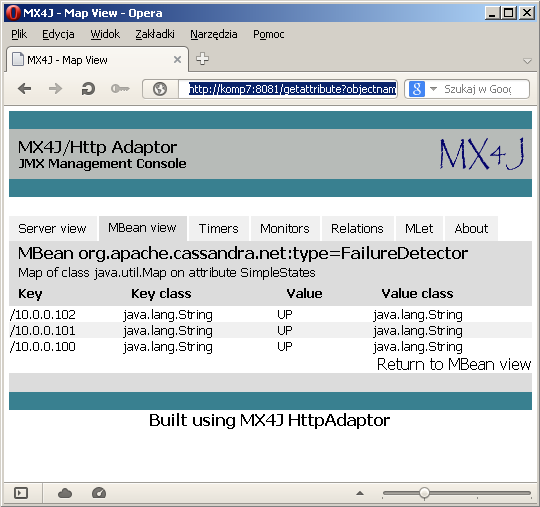
\includegraphics[width=0.8\linewidth]{gfx/mx4j-fd}
\caption{konsola \emph{MX4J}, podgląd stanu detektora awarii w węźle 10.0.0.100}
\label{fig:mx4j}
\end{figure}

\pagebreak

\noindent Oczywiście narzędzie \texttt{nodetool} także pozwala wyświetlić parametry pracy węzła:

\begin{lstlisting}[style=bash, columns=fixed, caption={statystyki dla puli wątków z~podziałem na zadania}]
$ nodetool -host localhost tpstats
Pool Name             Active Pending Completed Blocked Alltime blocked
ReadStage                  0       0         2       0               0
RequestResponseStage       0       0         2       0               0
MutationStage              0       0       122       0               0
ReadRepairStage            0       0         0       0               0
ReplicateOnWriteStage      0       0         0       0               0
GossipStage                0       0      4236       0               0
CacheCleanupExecutor       0       0         0       0               0
MigrationStage             0       0         0       0               0
MemoryMeter                0       0        13       0               0
FlushWriter                0       0         8       0               0
ValidationExecutor         0       0         0       0               0
InternalResponseStage      0       0         0       0               0
AntiEntropyStage           0       0         0       0               0
MemtablePostFlusher        0       0        42       0               0
MiscStage                  0       0         0       0               0
PendingRangeCalculator     0       0         5       0               0
CompactionExecutor         0       0        43       0               0
commitlog_archiver         0       0         0       0               0
HintedHandoff              0       0         2       0               0

Message type           Dropped
RANGE_SLICE                  0
READ_REPAIR                  0
PAGED_RANGE                  0
BINARY                       0
READ                         0
MUTATION                     0
_TRACE                       0
REQUEST_RESPONSE             0
COUNTER_MUTATION             0
\end{lstlisting}

\pagebreak

\begin{lstlisting}[style=bash, caption={statystyki dla przestrzeni kluczy \texttt{system\_auth}}]
$ nodetool -host localhost cfstats

[...]

Keyspace: system_auth
	Read Count: 2
	Read Latency: 43.764 ms.
	Write Count: 3
	Write Latency: 49.754 ms.
	Pending Tasks: 0

[...]

		Table: users
		SSTable count: 1
		Space used (live), bytes: 4689
		Space used (total), bytes: 4689
		SSTable Compression Ratio: 0.7611940298507462
		Number of keys (estimate): 128
		Memtable cell count: 0
		Memtable data size, bytes: 0
		Memtable switch count: 1
		Local read count: 1
		Local read latency: 0.000 ms
		Local write count: 1
		Local write latency: 0.000 ms
		Pending tasks: 0
		Bloom filter false positives: 0
		Bloom filter false ratio: 0.00000
		Bloom filter space used, bytes: 16
		Compacted partition minimum bytes: 61
		Compacted partition maximum bytes: 72
		Compacted partition mean bytes: 72
		Average live cells per slice (last five minutes): 1.0
		Average tombstones per slice (last five minutes): 0.0

----------------
\end{lstlisting}

\subsection{Przyłączanie i~odłączanie węzłów}\label{sec:management_nodepool}

By dodać do klastra nowy węzeł w~celu odciążenia pozostałych, należy wykonać procedurę analogiczną do opisanej w~punkcie \ref{subsec:cluster_connecting}.
Istnieje możliwość wyspecyfikowania w~pliku konfiguracyjnym za ile tokenów (a~nawet za jakie dokładnie) nowy węzeł będzie odpowiedzialny, ale nawet bez takiej informacji nowy węzeł będzie w~stanie skutecznie odciążyć klaster, ponieważ dzięki gossippingowi ma wgląd w~stan wszystkich innych węzłów.

Powodów by odłączyć węzeł może być kilka:
\begin{itemize}
\item klaster podlega aktualnie skalowaniu ,,w dół'' i~zbędne węzły są usuwane, choć cały czas działają prawidłowo
\item węzeł działa, choć niestabilnie~---~est spora szansa na to, że w najbliższym czasie ulegnie awarii, powinien więc być zastąpiony nowym
\item węzeł już uległ awarii i~nie odpowiada na zapytania, jednak inne węzły cały czas próbują się z~nim kontaktować
\end{itemize}

W~pierwszym przypadku węzeł można odłączyć przy pomocy procesu którego nazwę autorzy pozwolili sobie przetłumaczyć jako ,,złomowanie'' (\emph{ang.} decommissioning).
W~jego wyniku tokeny złomowanego węzła zostają usunięte z~pierścienia, a~dane, które się na nim znajdują są transferowane do nowych odpowiedzialnych za nie węzłów.

W~praktyce złomowanie węzła sprowadza się do wykonania jednego polecenia za pośrednictwem narzędzia \texttt{nodetool}:

\begin{lstlisting}[style=bash, caption={stan klastra z~perspektywy węzła w~nim pozostającego}]
$ nodetool status
Note: Ownership information does not include topology; for complete information,
specify a keyspace
Datacenter: DC1
===============
Status=Up/Down
|/ State=Normal/Leaving/Joining/Moving
--  Address     Load       Tokens  Owns   Host ID                               Rack
UN  10.0.0.101  115.51 KB  256     32.8%  d6537c65-2a7a-4359-a451-fdb4c6685b0c  NODE1AND2
UN  10.0.0.100  154.59 KB  256     35.0%  ac12364d-1ed1-4d8b-b667-0817f75dc065  NODE0
UN  10.0.0.102  115.33 KB  256     32.2%  ecdf71d2-1a4b-4727-bad6-8e293a0acbe3  NODE1AND2
\end{lstlisting}

\begin{lstlisting}[style=bash, caption={odłączenie węzła \texttt{NODE2}/10.0.0.102}]
$ nodetool decommission
\end{lstlisting}

\begin{lstlisting}[style=bash, caption={stan klastra z~perspektywy węzła w~nim pozostającego po odłączeniu węzła \texttt{NODE2}}]
$ nodetool status
Note: Ownership information does not include topology; for complete information,
specify a keyspace
Datacenter: DC1
===============
Status=Up/Down
|/ State=Normal/Leaving/Joining/Moving
--  Address     Load       Tokens  Owns   Host ID                               Rack
UN  10.0.0.101  125.02 KB  256     50.7%  d6537c65-2a7a-4359-a451-fdb4c6685b0c  NODE1AND2
UN  10.0.0.100  154.59 KB  256     49.3%  ac12364d-1ed1-4d8b-b667-0817f75dc065  NODE0
\end{lstlisting}

\bigskip

\noindent\textbf{UWAGA!} Żadne dane nie są usuwane ze złomowanego węzła, więc jeżeli ma on być ponownie wykorzystany w~innym miejscu pierścienia (z innym tokenem), należy wpierw opróżnić jego katalog danych ręcznie.

\bigskip

W~drugim przypadku może być potrzebna naprawa klastra po tymczasowej (\emph{ang.} transient) awarii węzła.
Standardowe mechanizmy zapewniania ostatecznej spójności są w~stanie rozwiązać problemy pojawiające się w~takiej sytuacji, z~jednym wyjątkiem.
Gdy awaria trwa dłużej niż wynosi okres życia \emph{tombstonów}, uszkodzony węzeł mógł nie zarejestrować pewnych operacji usunięcia wierszy.

Wtedy zaleca się wyczyszczenie węzła (usunięcie zawartości jego katalogu danych), usunięcie związanych z~nim tokenów z~pierścienia i~ponowne dodanie do klastra:

\pagebreak

\begin{lstlisting}[style=bash, caption={usuwanie węzła z~nieaktualnymi danymi z~klastra}]
$ nodetool ring

Datacenter: DC1
==========
Address     Rack      Status State   Load     Owns    Token
                                                      4960255647790084904
10.0.0.100  NODE0     Up     Normal  35.91 KB 81.40%  -8739202312123959326
10.0.0.101  NODE1AND2 Down     Normal  35.88 KB 44.33%  -5308254802912860692
10.0.0.102  NODE1AND2 Up     Normal  35.92 KB 74.26%  4960255647790084904

$ nodetool status
Datacenter: DC1
===============
Status=Up/Down
|/ State=Normal/Leaving/Joining/Moving
--  Address     Load       Tokens  Owns (effective)  Host ID                               Rack
DN  10.0.0.101  35.88 KB   1       44.3%             f329244e-c4ac-4fb0-8343-4476d97a311f  NODE1AND2
UN  10.0.0.100  35.91 KB   1       81.4%             ae935af3-d6b9-433a-a359-a6ef623340fe  NODE0
UN  10.0.0.102  35.92 KB   1       74.3%             b5c8225f-aff8-4e7d-9d82-221dc113adad  NODE1AND2

$ nodetool removenode f329244e-c4ac-4fb0-8343-4476d97a311f

$ nodetool status
Datacenter: DC1
===============
Status=Up/Down
|/ State=Normal/Leaving/Joining/Moving
--  Address     Load       Tokens  Owns (effective)  Host ID                               Rack
UN  10.0.0.100  35.91 KB   1       100.0%            ae935af3-d6b9-433a-a359-a6ef623340fe  NODE0
UN  10.0.0.102  35.92 KB   1       100.0%            b5c8225f-aff8-4e7d-9d82-221dc113adad  NODE1AND2

$ nodetool ring

Datacenter: DC1
==========
Address     Rack      Status State  Load     Owns    Token
                                                     4960255647790084904
10.0.0.100  NODE0     Up     Normal 35.91 KB 100.00% -8739202312123959326
10.0.0.102  NODE1AND2 Up     Normal 35.92 KB 100.00% 4960255647790084904
\end{lstlisting}

\bigskip

\noindent\textbf{UWAGA!} Różnica pomiędzy operacją \texttt{decommission} a~\texttt{removenode} jest taka, że druga z~nich zakłada że usuwany węzeł nie działa.
W~związku z~tym nowe węzły odpowiedzialne za zwalniany zakres tokenów będą pobierały dane z~pozostałych w~systemie replik, podczas gdy w~trakcie złomowania źródłem danych będzie złomowany węzeł.

\bigskip

Wreszcie w~przypadku całkowitej awarii węzła znaczącą rolę będzie miało opóźnienie odczytów i~zapisów związane z~,,problemami technicznymi'' i/lub niespójność danych.

Gdy każdy z~węzłów ma przydzielony tylko jeden token (przydzielany ręcznie), można ten problem rozwiązać następująco:
\begin{enumerate}
\item[1)] należy zastępczy węzeł odpowiednio przygotować poprzez nadanie mu adresu IP innego niż poprzednikowi i~tokenu mniejszego o~1 od tokenu poprzednika
\item[2)] podczas przyłączenia do klastra węzeł nie będzie odpowiadał na żądania odczytu aż do momentu zakończenia tego procesu
\item[3)] po przyłączeniu zastępcy martwy węzeł będzie odpowiadał tylko za jeden token~---~należy go usunąć z~pierścienia poleceniem \texttt{nodetool removetoken}
\item[4)] na każdym z~pozostałych węzłów należy wykonać polecenie \texttt{nodetool cleanup}, by uaktualnienia tam zapamiętane w~efekcie działania mechanizmu \emph{HintedHandoff} niepotrzebnie nie zajmowały miejsca~---~nigdy nie dotrą one do celu ponieważ węzeł, do którego były adresowane został trwale usunięty z~klastra
\end{enumerate}

W~przypadku standardowej konfiguracji (wiele tokenów dla pojedynczego węzła, dodatkowo przydzielanych automatycznie), procedura naprawy polega na podłączeniu zastępcy z~takim samym adresem IP i~uruchomieniu na nim polecenia \texttt{nodetool repair}.
Jest to o tyle kłopotliwe, że dla odczytów z~żądanym niskim poziomem spójności (np. ONE) węzeł przez okres naprawy (który może być bardzo długi) będzie zwracał klientom informację o~braku danych.

\pagebreak

\begin{thebibliography}{10}%===================================================

\bibitem[1]{facebook_paper}
A. Lakchman, P. Malik,\\
\emph{Cassandra~---~A~Decentralized Structured Storage System},\\
ACM SIGOPS Operating Systems Review,\\
Volume 44 Issue 2, April 2010

\bibitem[2]{prezentacja_srds}
Jan Baranowski, Michał Kaik, Maciej Urbański,\\
\emph{Cassandra, Highly available, scalable storage system},\\
Politechnika Poznańska 2014

\bibitem[3]{definitiveguide}
E. Hewitt,\\
\emph{Cassandra, The Defintive Guide},\\
O'Reilly 2010

\bibitem[4]{datastax}
\emph{DataStax},\\
\url{http://www.datastax.com/},\\
dostęp 17 czerwca 2014 r.

\bibitem[5]{debian_packaging}
\emph{DebianPackaging, Cassandra Wiki},\\
\url{https://wiki.apache.org/cassandra/DebianPackaging}.\\
dostęp 16 czerwca 2014 r.

\bibitem[6]{distributeddeletes}
\emph{DistributedDeletes, Cassandra Wiki},\\
\url{http://wiki.apache.org/cassandra/DistributedDeletes}\\
dostęp 17 czerwca 2014 r.

\bibitem[7]{ganglia}
\emph{Ganglia Monitoring System},
\url{http://ganglia.sourceforge.net/}\\
dostęp 18 czerwca 2014 r.

\bibitem[8]{getting_started}
\emph{GettingStarted, Cassandra Wiki},\\
\url{http://wiki.apache.org/cassandra/GettingStarted},\\
dostęp 16 czerwca 2014 r.

\bibitem[9]{downloading_oracle_java}
Daniel Stavrovski,\\
\emph{Installing Oracle JAVA 7 on Debian Wheezy},\\
\url{http://d.stavrovski.net/blog/post/installing-oracle-java-7-on-debian-wheezy},\\
dostęp 16 czerwca 2014 r.

\bibitem[10]{installing_oracle_java_on_debian}
\emph{Java/Sun, Debian Wiki},\\
\url{https://wiki.debian.org/Java/Sun},\\
dostęp 16 czerwca 2014 r.

\bibitem[11]{mysql_connectors}
\emph{MySQL Connectors},\\
\url{http://www.mysql.com/products/connector/},\\
dostęp 16 czerwca 2014 r.

\bibitem[12]{datastax_guides}
\emph{NoSQL Apache Cassandra Documentation},\\
\url{http://planetcassandra.org/documentation/},\\
dostęp 16 czerwca 2014 r.

\bibitem[13]{ntp}
\emph{NTP, Debian Wiki},\\
\url{https://wiki.debian.org/NTP},\\
dostęp 16 czerwca 2014 r.

\bibitem[14]{cluster_operations}
\emph{Operations, Cassandra Wiki},\\
\url{http://wiki.apache.org/cassandra/Operations},\\
dostęp 16 czerwca 2014 r.

\bibitem[15]{whydatastax}
\emph{Why DataStax?},\\
\url{http://www.datastax.com/why-datastax}\\
dostęp 16 czerwca 2014 r.

\end{thebibliography}

\end{document}